%!TEX TS-program = xelatex
%!TEX encoding = UTF-8 Unicode

\documentclass[11pt,tikz,border=1]{standalone}
\usetikzlibrary{positioning,decorations.pathreplacing}

\begin{document}
  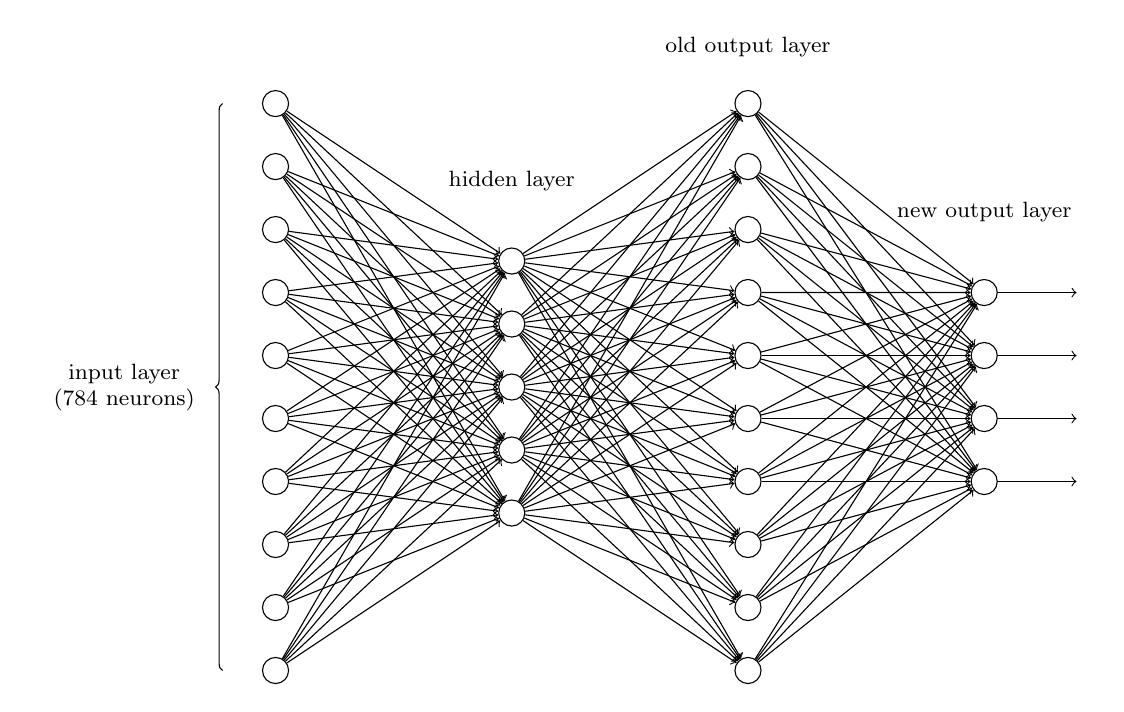
\begin{tikzpicture}[
    neuron/.style={circle,draw,inner sep=0pt,minimum size=5mm},
    font=\footnotesize
    ]

      % leftmost layer, 10 nodes:
      \foreach \y in {0,...,9}
      \node (l\y) at (-3, \y / 1.25) [circle,draw] {};

      % hidden layer, 5 nodes:
      \foreach \y in {0,...,4}
      \node (m\y) at (0, 2 + \y / 1.25) [circle,draw] {};

      % old output layer, 10 nodes:
      \foreach \y in {0,...,9}
      \node (r\y) at (3, \y / 1.25) [circle,draw] {};

      % new output layer, 4 nodes:
      \foreach \y in {0,...,3}
      \node (o\y) at (6, 2.4 + \y / 1.25) [circle,draw] {};

      % new output layer, 4 nodes:

      \foreach \y in {0,...,3}
      \node (a\y) [right=of o\y] {};

      \begin{scope}[node distance=3mm]
	      \node (text2) [above=of r9] {
          old output layer
	       };
      \end{scope}

      \begin{scope}[node distance=6mm]
        \node (text1) [above=of m4] {
          hidden layer
        };
        \node (text3) [above=of o3] {
          new output layer
        };
      \end{scope}

      % draw brace:
      \draw[decorate,decoration={brace,mirror}] ([xshift=-5mm]l9.west) -- ([xshift=-5mm]l0.west) node [midway,xshift=-12.5mm] {
        \begin{tabular}{c}
          input layer \\
          ($784$ neurons)
    	\end{tabular}
      };

      % connections:
      \foreach \x in {0,...,9}
      \foreach \y in {0,...,4}
      \draw [->] (l\x) to (m\y);

      \foreach \x in {0,...,4}
      \foreach \y in {0,...,9}
      \draw [->] (m\x) to (r\y);

      \foreach \x in {0,...,9}
      \foreach \y in {0,...,3}
      \draw [->] (r\x) to (o\y);

      \foreach \x in {0,...,3}
      \draw [->] (o\x) to (a\x);

  \end{tikzpicture} 
\end{document}
